\subsubsection{Luftflöde genom väggar – drag}

\begin{figure}[hpbt]
\centering
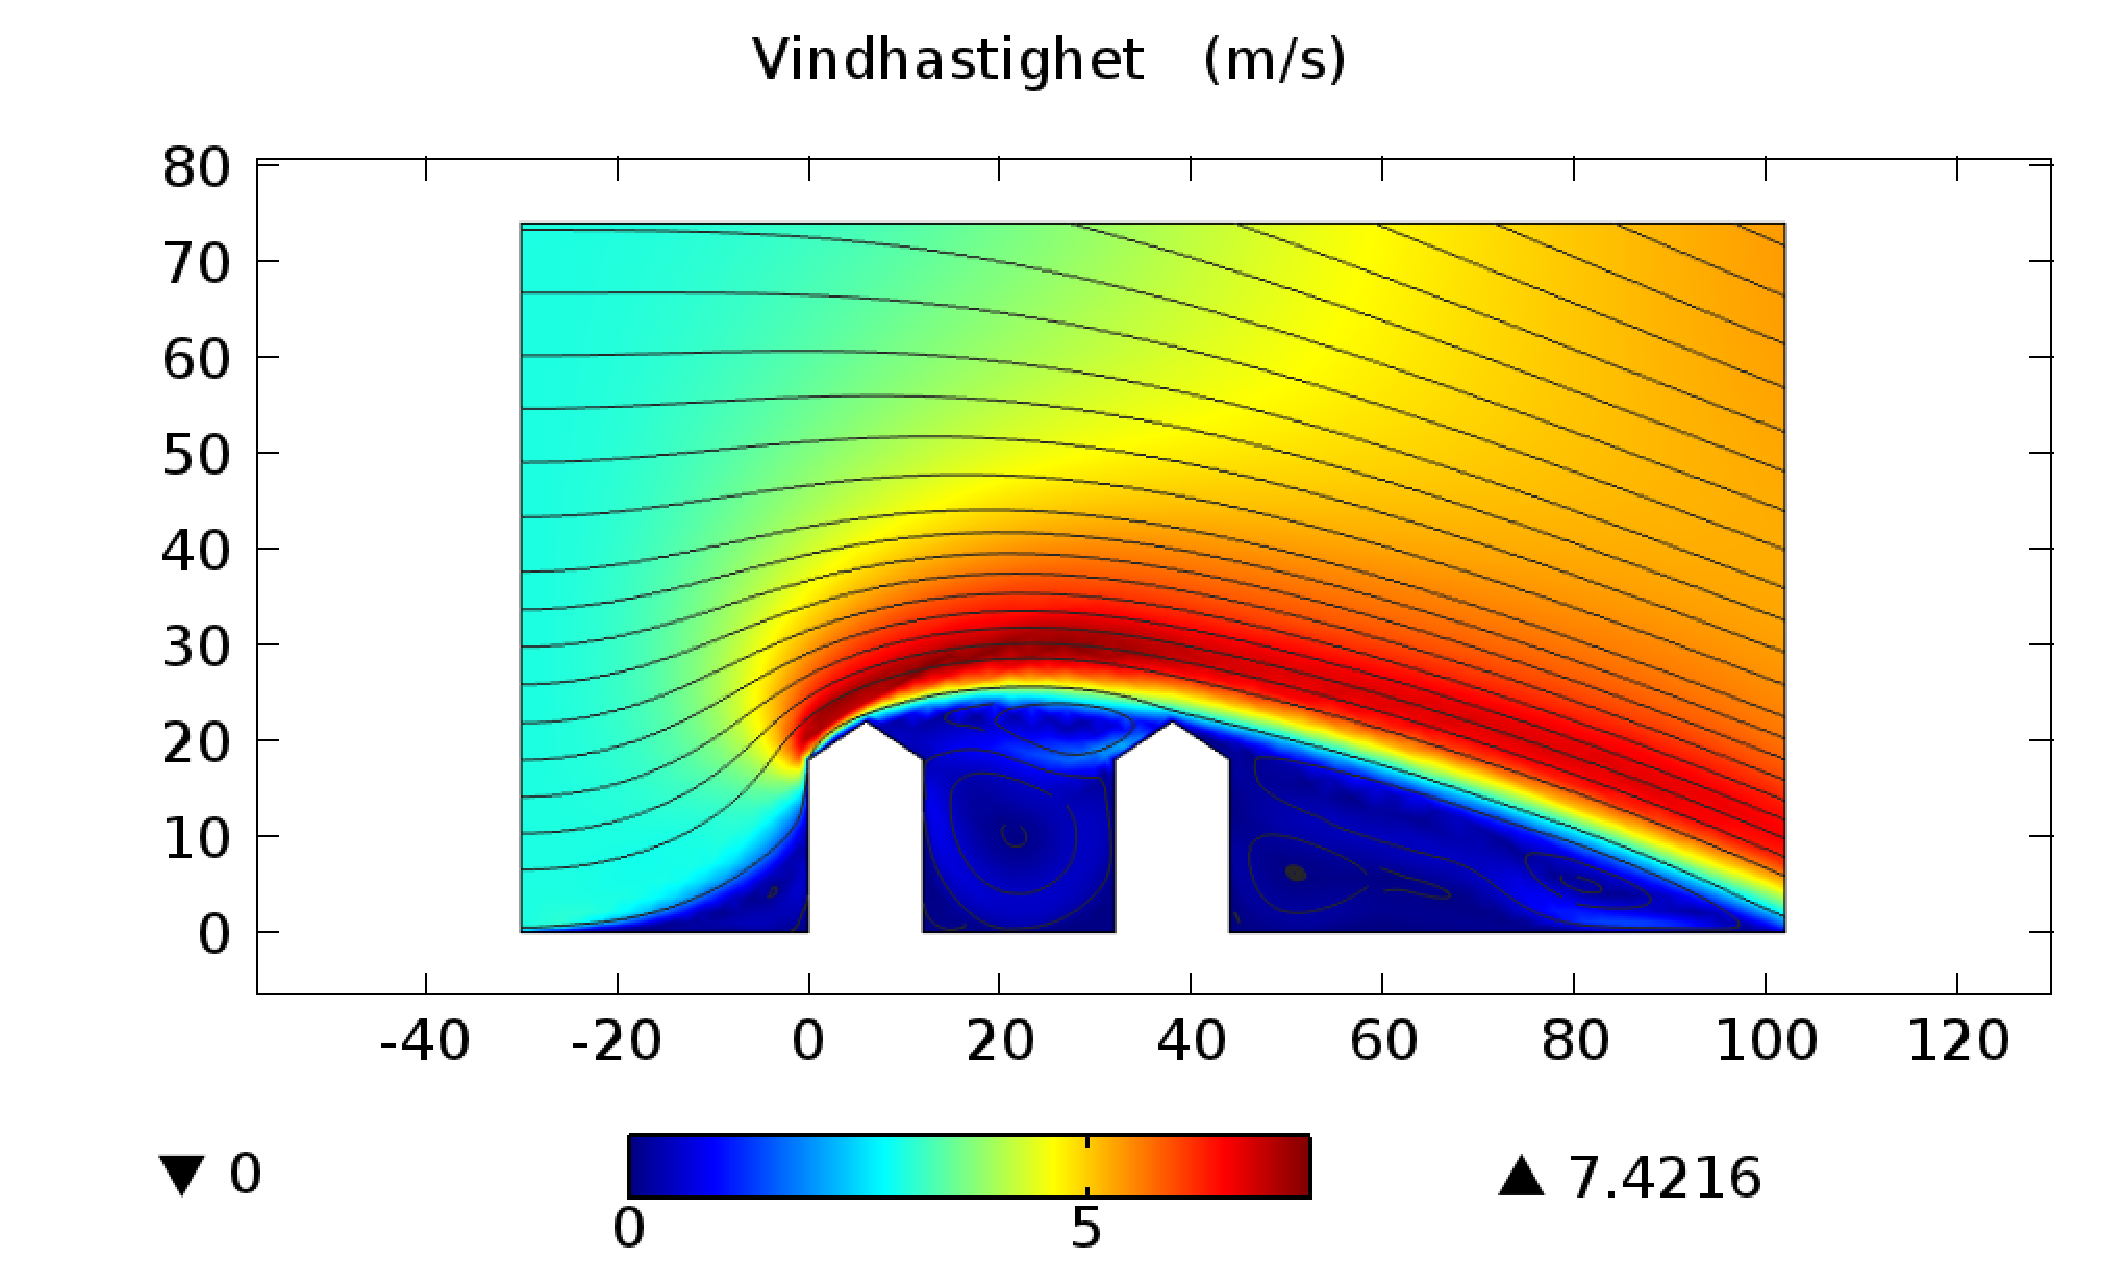
\includegraphics[width=130mm,height=78mm]{images/wind3mshdpi.eps}
\caption{Vindhastiheten när vind i $\unit[3]{ m/s}$ blåser mot fastigheten. Linjerna
i figuren är strömlinjer och färgen indikerar beloppet av hastighetsvektorn. Värdena är framräknade med Comsol.\emph{\color{red} Nu är dessa bilder i 200dpi. Borde jag byta till ännu högre?}}
\end{figure}

\begin{figure}[hpbt]
\centering
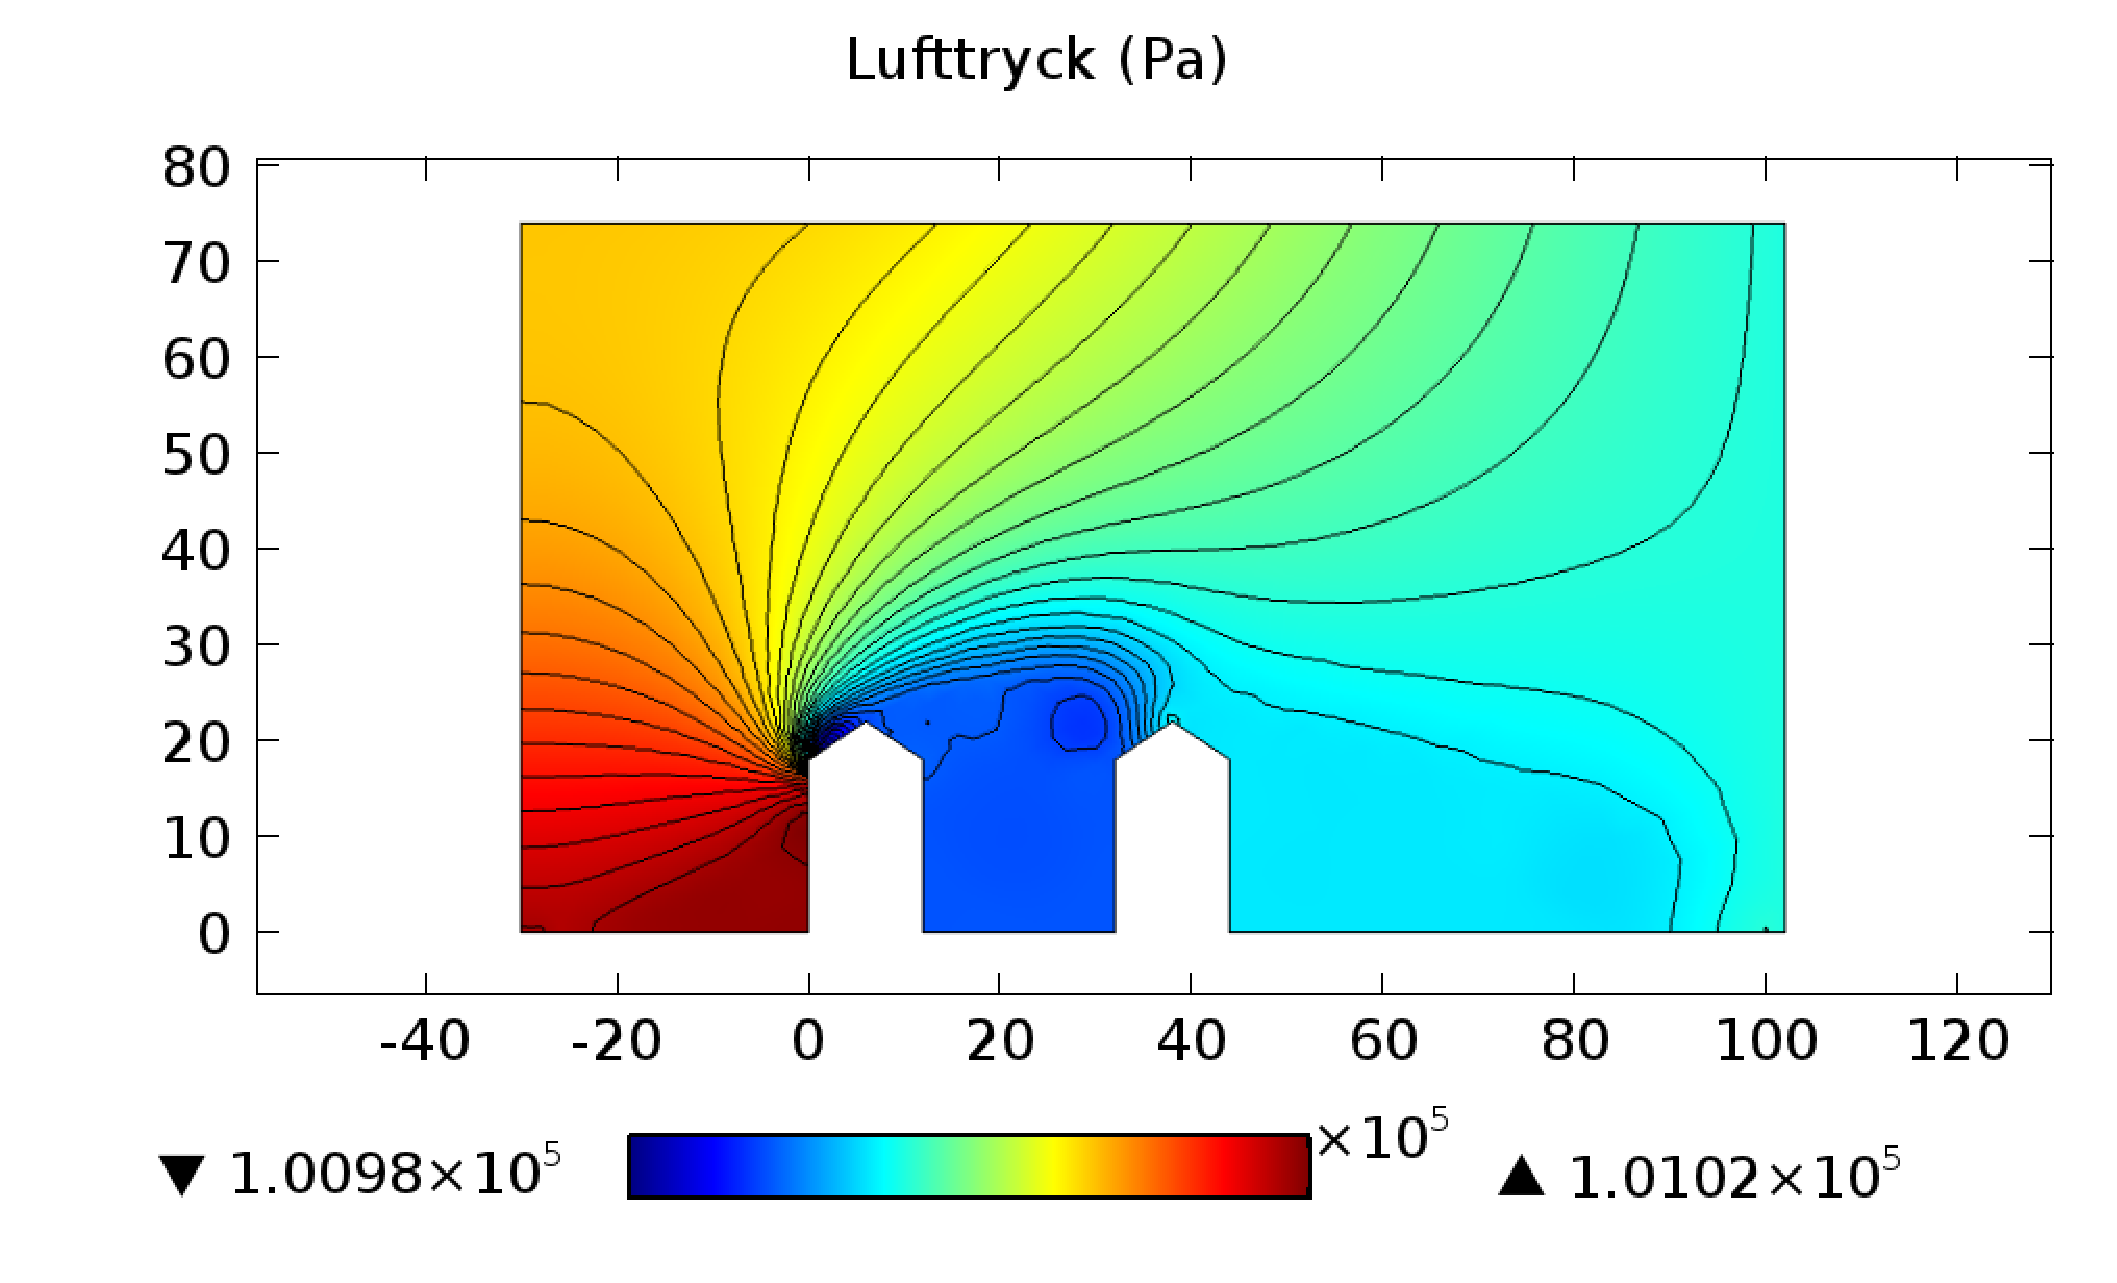
\includegraphics[width=130mm,height=78mm]{images/pressure3mshdpi.eps}
\caption{Lufttrycket när vind i $\unit[3]{ m/s}$ blåser från vänster
sida i figuren. Färgen indikerar lufttryck och linjer ligger längs isobarer.
Tryckskillnaderna på de olika sidorna av husen kommer att driva ofrivillig ventilation vilket leder till infiltrationsförluster.\emph{\color{red} Nu är dessa bilder i 200dpi. Borde jag byta till ännu högre?}}
\end{figure}


\begin{figure}[hpbt]
\centering
\subfloat[Byggnad som vinden blåser direkt på.]{
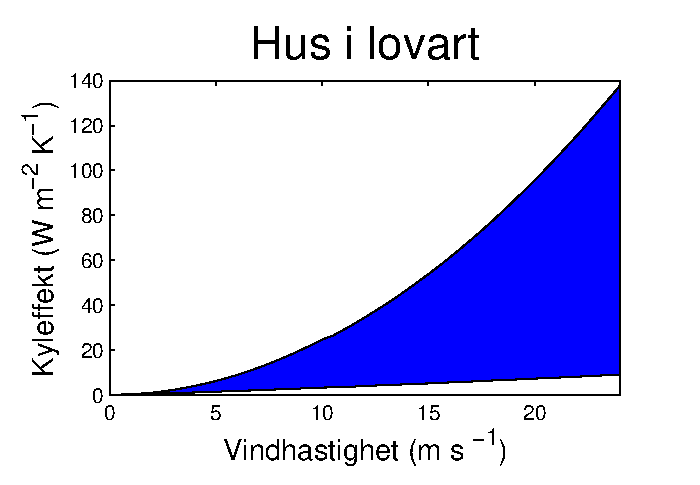
\includegraphics[width=60mm]{images/pressurewind.eps}}
\vspace{5mm}
\subfloat[Byggnad som ligger i lä av en annan byggnad.]{
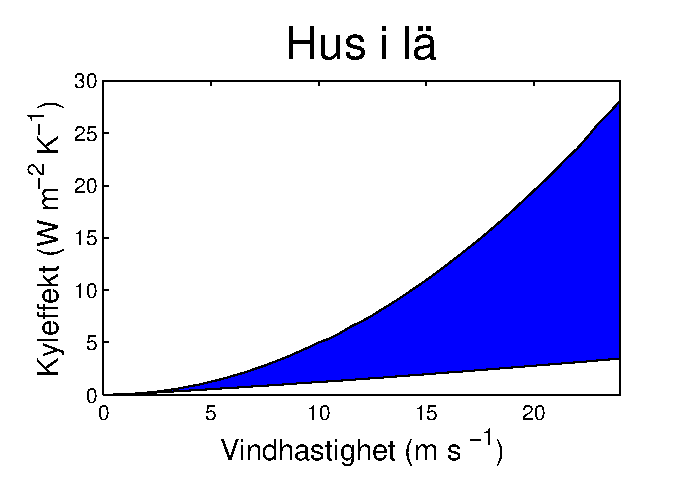
\includegraphics[width=60mm]{images/pressurenowind.eps}}

\subfloat[Teoretisk approximation för lådformad byggnad.]{
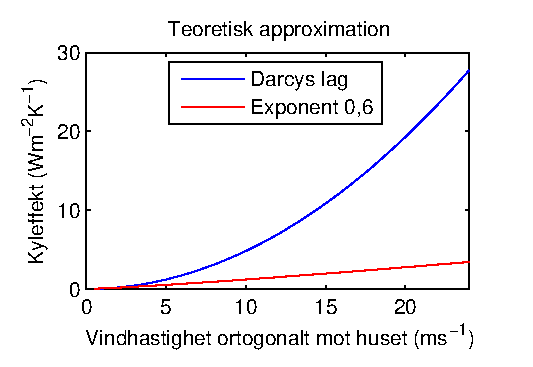
\includegraphics[width=60mm]{images/pressuretheory.eps}}
\caption{Energiförlust per temperaturenhet med exponent 1 vilket motsvarar
Darcys lag och med exponent $0,6$ vilket är en experimentellt uppmätt
exponent. Dessa två kurvor kan motsvara högsta och minstagissningar för
infiltrationsförluster i en byggnad. Trycken är framräknade för olika
vindhsatigheter med Comsol och andra är teoretiskt framräknade med en approximation.
Denna baserar sig på att tryckskillnaden mellan inne och ute är proportionerligt
med vindhastiheten i kvadrat.}
\end{figure}
